\documentclass{article}


% if you need to pass options to natbib, use, e.g.:
%     \PassOptionsToPackage{numbers, compress}{natbib}
% before loading neurips_2023


% ready for submission
\usepackage[final,nonatbib]{neurips_2023}

 \usepackage{amsmath}
% to compile a preprint version, e.g., for submission to arXiv, add add the
% [preprint] option:
%     \usepackage[preprint]{neurips_2023}


% to compile a camera-ready version, add the [final] option, e.g.:
%     \usepackage[final]{neurips_2023}


% to avoid loading the natbib package, add option nonatbib:
%    \usepackage[nonatbib]{neurips_2023}


\usepackage[utf8]{inputenc} % allow utf-8 input
\usepackage[T1]{fontenc}    % use 8-bit T1 fonts
\usepackage{hyperref}       % hyperlinks
\usepackage{url}            % simple URL typesetting
\usepackage{booktabs}       % professional-quality tables
\usepackage{amsfonts}       % blackboard math symbols
\usepackage{nicefrac}       % compact symbols for 1/2, etc.
\usepackage{microtype}      % microtypography
\usepackage{xcolor}         % colors
\usepackage{graphicx}
\usepackage{float}
\usepackage{tabularx}
\usepackage[square,numbers]{natbib}
\bibliographystyle{agsm}
\usepackage{pdfpages}

\title{CPSC 577 Project Report\\Enhancing Text Classification with GraphSAGE}


% The \author macro works with any number of authors. There are two commands
% used to separate the names and addresses of multiple authors: \And and \AND.
%
% Using \And between authors leaves it to LaTeX to determine where to break the
% lines. Using \AND forces a line break at that point. So, if LaTeX puts 3 of 4
% authors names on the first line, and the last on the second line, try using
% \AND instead of \And before the third author name.



\author{%
  Shurui Wang \\
  \texttt{shurui.wang@yale.edu} \\
  % examples of more authors
  \And
  Weiyi You \\
  \texttt{weiyi.you@yale.edu} \\
  \And
  Lang Ding \\
  \texttt{lang.ding@yale.edu} \\
}

\begin{document}


\maketitle
\begin{abstract}
  This project explores the enhancement of text classification through the novel application of TextGraphSAGE, a graph-based neural network model that integrates textual and relational data. By constructing text graphs at a granular level with nodes representing individual words or phrases and edges reflecting adjacency, we aim to capture both local and global textual contexts more effectively. The project compares the performance of our TextGraphSAGE model with conventional deep learning models like CNNs and LSTMs, as well as another graph-based method, TextGCN, across two datasets: Reuters R8 and Twitter Asian Prejudice. Our results indicate that TextGraphSAGE outperforms the baseline models, demonstrating its potential to leverage relational information for superior text classification accuracy and efficiency. Our findings affirm the potential of graph-based methods in advancing text classification tasks. Code is available at \href{https://github.com/JadenWSR/TextGraphSAGE}{https://github.com/JadenWSR/TextGraphSAGE}.
\end{abstract}
\section{Introduction and Motivation}

Text classification is a foundational task in Natural Language Processing (NLP) aimed at assigning one or more categories to a piece of text. Traditional approaches range from rule-based to advanced deep learning techniques. Recently, the application of graph-based models like Graph Neural Networks (GNNs) has shown promising results in various NLP tasks, including text classification. These models, particularly GraphSAGE (Graph Sample and Aggregate), offer a novel approach to incorporate not just the textual information but also the relational context within a document.

\section{Problem Definition}

While traditional deep learning models for text classification have achieved impressive results, they often neglect the rich relational information available in textual datasets. This information includes implicit connections between words and entities within a document. GraphSAGE presents an opportunity to leverage this relational information by learning representations that incorporate both the content of documents and their context within a graph structure. This project aims to explore how GraphSAGE can be utilized to enhance text classification by effectively integrating textual and relational information.

\section{Related Work}

The application of graph-based methods in text classification has emerged as a significant advancement in NLP, addressing limitations of conventional models that fail to capture the complex relational structure of text data. Text Graph Convolutional Networks (Text GCN) introduced by Yao et al. \cite{Yao2018GraphCN} pioneered the integration of document and word nodes within a single graph, leveraging graph convolutional networks for enhanced text classification. This method, while innovative, constructs a static graph from the entire corpus, potentially limiting its adaptability and scalability for large datasets or dynamic text streams.

GraphSAGE, proposed by Hamilton et al. \cite{Hamilton2017GraphSAGE}, offers a flexible framework for inductive representation learning on graphs. By sampling and aggregating features from a node's local neighborhood, GraphSAGE generates embeddings that encapsulate both local structure and node-level features, enabling efficient learning on large, dynamic graphs. This approach's adaptability and efficiency in handling relational data make it a promising foundation for our proposed method.

Convolutional Neural Networks (CNN) and Long Short-Term Memory networks (LSTM) have also been extensively applied in text classification, showcasing the power of deep learning models in capturing semantic patterns and dependencies within text \cite{Kim2014CNN, Liu2016RNN}. However, these models often overlook the relational information embedded in the text's graph structure, a gap our project aims to bridge by leveraging GraphSAGE's capability to integrate textual and relational data.

Our project aims to bridge the gap between traditional deep learning models, such as CNNs \cite{Kim2014CNN} and LSTMs \cite{Liu2016RNN}, and graph-based approaches by employing GraphSAGE for text classification. Our proposed approach distinguishes itself by constructing a text graph at a granular level, where nodes represent individual words or phrases, and edges reflect adjacency within a window. This novel application of GraphSAGE for text classification aims to capture both local and global textual contexts, promising improvements in classification accuracy and efficiency over existing models.


\section{Method}

We proposed a custom GraphSAGE implementation, TextGraphSAGE, to construct and analyze text graphs, where nodes represent words and documents.

\subsection{Model Framework and Mathematical Setting}

\subsubsection{GraphSAGE}
GraphSAGE, or Graph Sample and Aggregated Embeddings, is a method that learns continuous vector representations of nodes in a graph, capturing both structural and contextual information about each node \cite{Hamilton2017GraphSAGE}. This inductive learning approach allows GraphSAGE to generate embeddings for previously unseen nodes during training by iteratively sampling and aggregating information from a node's local neighborhood.

The function of GraphSAGE is described as follows:
\begin{equation}
h_v^{(l)} = \sigma \left( W^{(l)} \text{CONCAT} \left( h_v^{(l-1)}, \text{AGG}\left( \{h_u^{(l-1)}, u \in N(v)\} \right) \right) \right)
\end{equation}

Aggregation occurs in two stages:
\begin{itemize}
    \item Stage 1: Aggregate from neighboring nodes:
    \begin{equation}
    h_{N(v)}^{(l)} = \text{AGG}\left( \{h_u^{(l-1)}, u \in N(v)\} \right)
    \end{equation}

    \item Stage 2: Combine the node's own features:
    \begin{equation}
    h_v^{(l)} = \sigma \left( W^{(l)} \text{CONCAT} \left( h_v^{(l-1)}, h_{N(v)}^{(l)} \right) \right)
    \end{equation}
\end{itemize}

where $h_{N(v)}^{(l)}$ represents the hidden layer representation of node $v$ at layer $l$, $W^{(l)}$ is the weight matrix for neighborhood aggregation, and $N(v)$ represents the neighborhood of node $v$. AGG denotes the aggregation function, which can be mean, pooling, or an LSTM approach for order-sensitive aggregation.

\subsubsection{TF-IDF and PMI}
\begin{itemize}
    \item TF-IDF: Term Frequency-Inverse Document Frequency (TF-IDF) weights are used for the edges linking documents to words within the graph. The TF-IDF value is calculated as follows:
    \begin{equation}
    w_{t,d} = tf_{t,d} \times idf_t
    \end{equation}
    where $tf_{t,d} = \text{count}(t, d)$ is the term frequency and $idf_t = \log_{10} \left(\frac{N}{df_t}\right)$, with $df_t$ representing the number of documents containing term $t$.

    \item PMI: Pointwise Mutual Information (PMI) assesses the co-occurrence strength of word pairs above that expected by chance and is used to weight word-word edges in the graph:
    \begin{equation}
    PMI(X,Y) = \log_2 \left( \frac{P(x,y)}{P(x)P(y)} \right)
    \end{equation}
    where $p(x,y) = \frac{\#W(x, y)}{\#W}$ and $p(x) = \frac{\#W(x)}{\#W}$. Only positive PMI values are used, indicating a significant semantic correlation between the word pairs.
\end{itemize}

\subsection{TextGraphSAGE}

TextGraphSAGE integrates the principles of GraphSAGE into a text classification framework by building a heterogeneous graph composed of both word and document nodes. This graph effectively models global co-occurrence and contextual relationships within texts, leveraging node and edge features optimized for text data.

\begin{enumerate}
    \item \textbf{Text Graph Construction}: 
    A graph is constructed where each node represents either a word or a document, forming a comprehensive network that maps the intricate relationships and frequencies of word occurrences across documents.
    \item \textbf{Node Embedding}: Utilizing identity matrices, each node (word or document) is represented by a distinct one-hot vector, which is then enhanced through embeddings derived from pre-trained models to encode semantic information.
    \item \textbf{Edge Weighting}: Edges between document and word nodes are weighted by TF-IDF to emphasize word relevance in documents, while edges between words are weighted by PMI to capture the semantic similarity based on their co-occurrence within specific contexts.
    \item \textbf{Neighborhood Aggregation}: Adopts a two-layer GraphSAGE network with a softmax classifier to process node embeddings, utilizing sum aggregation to capture textual context from node neighborhoods effectively.
    \item \textbf{Aggregation Strategy}: Implements dense matrix multiplication for sum aggregation, optimizing the model for efficient GPU usage.
\end{enumerate}


This approach not only preserves the local and global semantic relationships inherent in text data but also enhances the adaptability and efficacy of the model by integrating GraphSAGE's inductive learning capabilities, allowing it to handle unseen data effectively.

\subsection{Baseline Models}

Our evaluation will compare the proposed approach against several established models:

\begin{enumerate}

     \item Convolutional Neural Network (CNN) \cite{Kim2014CNN}, which employs randomly initialized word embeddings for its architecture, focusing on the CNN-rand variant.
    
    \item Long Short-Term Memory network (LSTM) \cite{Liu2016RNN}, which uses the last hidden state to encapsulate the entire text representation, focusing on the model's ability to capture long-term dependencies.
    
    \item Text Graph Convolutional Networks (Text GCN) \cite{Yao2018GraphCN}, which constructs a large graph from the entire corpus, representing both words and documents as nodes. This approach utilizes a two-layer Graph    
\end{enumerate}

\section{Experiments}
\subsection{Computing Infrastructure}

Our computing environment for training and testing the models included using a single T4 GPU on Google Colab for the baseline models (CNN, LSTM, and TextGCN) and a single GPU on the YALE cluster for the TextGraphSAGE model. The specific configurations for TextGraphSAGE were managed using the `cpsc577\_env.yaml` environment setup available on our GitHub. Consistency in training and testing across all models was maintained by using the same 8/1/1 tvt split, but with different randomly chosen seeds [33, 15, 86, 109, 78] to ensure robustness and repeatability in results. Models were optimized using CrossEntropyLoss and the Adam optimizer configured with varying learning rates as determined by the hyperparameter tuning process.

\subsection{Hyperparameters and Tuning Process}

For the TextGraphSAGE model, we conducted hyperparameter tuning on both the R8 and Twitter datasets using a grid search approach. Hyperparameter tuning was performed with a seed of 123 and an 8/1/1 train/validation/test split. This tvt split allowed us to methodically fine-tune hyperparameters based on validation performance, ensuring that the best model parameters were used for final testing to achieve unbiased and generalizable results. The parameters considered include learning rate (`lr`) with options [0.01, 0.001, 0.0001], prediction type (`pred\_type`) with options ['softmax', 'mlp'], the presence of dropout (`dropout`) with options [True, False], and activation function (`act`) with options ['relu', 'prelu', 'sigmoid', 'tanh']. The best-performing parameters identified were for the R8 dataset: learning rate of 0.01, softmax prediction, no dropout, and PReLU activation; for the Twitter dataset: learning rate of 0.001, softmax prediction, no dropout, and tanh activation. Additional parameters such as word window size (10), validation window size (10), number of layers (2), and the use of CrossEntropyLoss and Adam optimizer, were kept consistent with the configurations found in the TextGCN paper\cite{Yao2018GraphCN}, as these settings yielded optimal results in preliminary experiments. For baseline models, default parameters from their original papers\cite{Kim2014CNN, Liu2016RNN, Yao2018GraphCN} or implementations were used without further tuning.

\subsection{Datasets} 

We employ two primary datasets in our study:

1. Reuters R8 Dataset\cite{r8}: This subset of the Reuters 21578 collection contains documents from 1987 newswire articles, divided into 8 categories: trade, ship, interest, earn, crude, money-fx, grain, and acquisition. The dataset consists of 5,485 training texts and 2,189 testing texts. Preprocessing involves standard text cleaning techniques such as removing stop words and infrequent words, and applying normalization steps to prepare the text for the graph-based model.

2. Twitter Asian Prejudice Dataset\cite{vidgen2020detecting}: Comprising 20,000 tweets related to East Asian prejudice, this dataset is categorized into five labels reflecting the nature of the tweets, including discussions on prejudice, counter-speech, and entity-directed hostility. Similar preprocessing steps are used here, tailored to handle social media text characteristics like hashtags and mentions.

Both datasets are publicly accessible through the Text-GCN repository on GitHub \href{https://github.com/codeKgu/Text-GCN/tree/master/data/corpus}{https://github.com/codeKgu/Text-GCN/tree/master/data/corpus}. For CNN and LSTM models, standard NLP data cleaning protocols are applied, including tokenization and filtering non-lexical items. For the TextGCN and TextGraphSAGE models, texts are further processed into a graph format as described in Section 4.2. This involves converting texts to nodes and edges in a graph, utilizing term frequency and document co-occurrence to weight the connections between nodes, thereby retaining semantic relationships within the data.


\subsection{Evaluation Metric}

In assessing the performance of TextGraphSAGE compared to baseline models(CNN, LSTM, and Text GCN), we employ three key metrics: accuracy, F1 macro, and F1 weighted. Accuracy provides a straightforward measure of overall model performance, indicating the proportion of total correct predictions across all classes. F1 macro is used to calculate the average effectiveness of the model across all classes, ensuring that each class is equally considered regardless of its frequency in the dataset. This is crucial for evaluating performance in datasets with imbalanced class distributions. F1 weighted offers a performance measure that accounts for class size, giving more weight to classes with more instances. This metric helps assess the model's effectiveness in handling class imbalance by reflecting the importance of each class based on its prevalence. These metrics collectively provide a comprehensive view of model performance, crucial for validating the enhancements offered by TextGraphSAGE over traditional text classification approaches.


\section{Results}

\begin{table}[H]
\centering
\caption{Performance on R8 Dataset}
\label{table:R8-results}
\begin{tabular}{lccc}
\hline
\textbf{Model} & \textbf{Accuracy} & \textbf{F1 Macro} & \textbf{F1 Weighted} \\ \hline
CNN &  0.8659$\pm$0.0715 & 0.5464$\pm$0.1751 & 0.8399$\pm$0.0963\\
LSTM & 0.8482$\pm$0.0402 & 0.5028$\pm$0.1018 & 0.8321$\pm$0.0495  \\
TextGCN & 0.9582$\pm$0.0027& 0.8795$\pm$0.0101 & 0.9586$\pm$0.0026 \\
TextGraphSAGE & \textbf{0.9630$\pm$0.0018} & \textbf{0.8998$\pm$0.0056} & \textbf{0.9633$\pm$0.0017} \\ \hline
\end{tabular}
\end{table}

\begin{table}[H]
\centering
\caption{Performance on Twitter Asian Prejudice Dataset}
\label{table:Twitter-results}
\begin{tabular}{lccc}
\hline
\textbf{Model} & \textbf{Accuracy} & \textbf{F1 Macro} & \textbf{F1 Weighted} \\ \hline
CNN & 0.6787$\pm$0.0073 & 0.1659 $\pm$ 0.0034 & 0.5540$\pm$0.0105 \\
LSTM & 0.6813$\pm$0.0078 & 0.1621$\pm$0.0011 & 0.5522$\pm$0.0100 \\
TextGCN & 0.7032$\pm$0.0264  & \textbf{0.5276$\pm$0.0200} & 0.7129$\pm$0.0193 \\
TextGraphSAGE & \textbf{0.7359$\pm$0.0090} & 0.5170$\pm$0.0337& \textbf{0.7133$\pm$0.0283} \\ \hline
\end{tabular}
\end{table}


\section{Conclusion \& Discussion}

The evaluation of the TextGraphSAGE model across two distinct datasets reveals its robust performance in text classification tasks. On the R8 dataset, TextGraphSAGE achieved an impressive accuracy of 0.9630±0.0018, surpassing the baseline models. It also demonstrated strong capability in balancing class representation, as indicated by its F1 Macro score of 0.8998±0.0056, and effectively managed class size variances, achieving an F1 Weighted score of 0.9633±0.0017. Performance on the Twitter Asian Prejudice dataset followed a similar trend, with TextGraphSAGE outperforming other models with an accuracy of 0.7359±0.0090. While the F1 Macro and F1 Weighted scores were slightly lower in this dataset at 0.5170±0.0337 and 0.7133±0.0283 respectively, they still represent competitive results, considering the challenging nature of classifying nuanced social media content. These results confirm TextGraphSAGE's effectiveness in leveraging both global and local textual contexts, significantly enhancing text classification outcomes compared to conventional methods.



\subsection{Limitations}
\subsubsection{Positional information}
Our graph-based model converts words and documents into nodes linked by edges weighted with TF-IDF or PMI, which inherently lacks explicit positional information. This absence means there is no inherent order to the nodes that correspond to their original sequence in the text, potentially resulting in ambiguous or inconsistent interpretations of node positions. Although positional information could be simulated in edge weighting, it does not naturally capture the sequential flow of text as in traditional NLP models.

\subsubsection{Long-range Dependencies}

TextGraphSAGE focuses on local node neighborhoods, which might restrict its capability to model long-range dependencies crucial for understanding broader textual contexts. Although attention mechanisms can partly mitigate this limitation, effectively capturing extended dependencies between distant words or across document sections remains a substantial challenge for our graph-based approach.

\subsubsection{Dynamic Text Data}
Text data is often dynamic in real world problem, with new words, documents, or concepts being introduced over time. Adapting a graph-structured neural network to dynamically changing text data while efficiently updating the model parameters can be challenging, especially in scenarios with streaming or evolving text data.

\subsection{Future Work}
There is a lot of room for improvement of our model and idea.
\subsubsection{Incorporating Positional Information}
Future enhancements could include developing methods to integrate positional information into the TextGraphSAGE framework. This could involve novel positional encoding techniques or graph architectures that explicitly account for the hierarchical or sequential structure of textual data, potentially improving the model's natural language processing capabilities.

\subsubsection{Dynamic graph adaptation}
Further research could explore adaptive strategies for TextGraphSAGE to handle dynamically changing text data. This would support more robust applications in streaming or continuously updated document sets, enhancing the model’s practicality in dynamic environments.

\subsubsection{Semantic Graph Augmentation}
Enhancing text graph representations with external semantic knowledge, such as incorporating data from knowledge graphs or ontologies, could significantly boost the semantic interpretation capabilities of our model. Investigating automated methods for semantic graph augmentation and leveraging this enriched information during model training and inference could provide substantial advancements. Additionally, exploring transitions to other models like Transformers could offer improved handling of long-range dependencies.


\newpage
\section{Contribution Statement}

All members of our group collaborated to conceptualize and execute the project. Weiyi was responsible for the datasets; he preprocessed and cleaned them to ensure compatibility with different models. Lang focused on constructing the text graphs, namely transferring text data to a graph. Shurui designed the TextGraphSAGE structure. Regarding model implementation, Weiyi developed the CNN baseline model, Lang worked on the LSTM baseline model, and Shurui both trained the TextGCN baseline model and performed hyperparameter tuning for the TextGraphSAGE model. For the project report, Weiyi authored Sections 1, 2, and 7; Lang contributed to Sections 3 and 4; and Shurui wrote Sections 5 and 6.


\small
\bibliography{reference}
\newpage
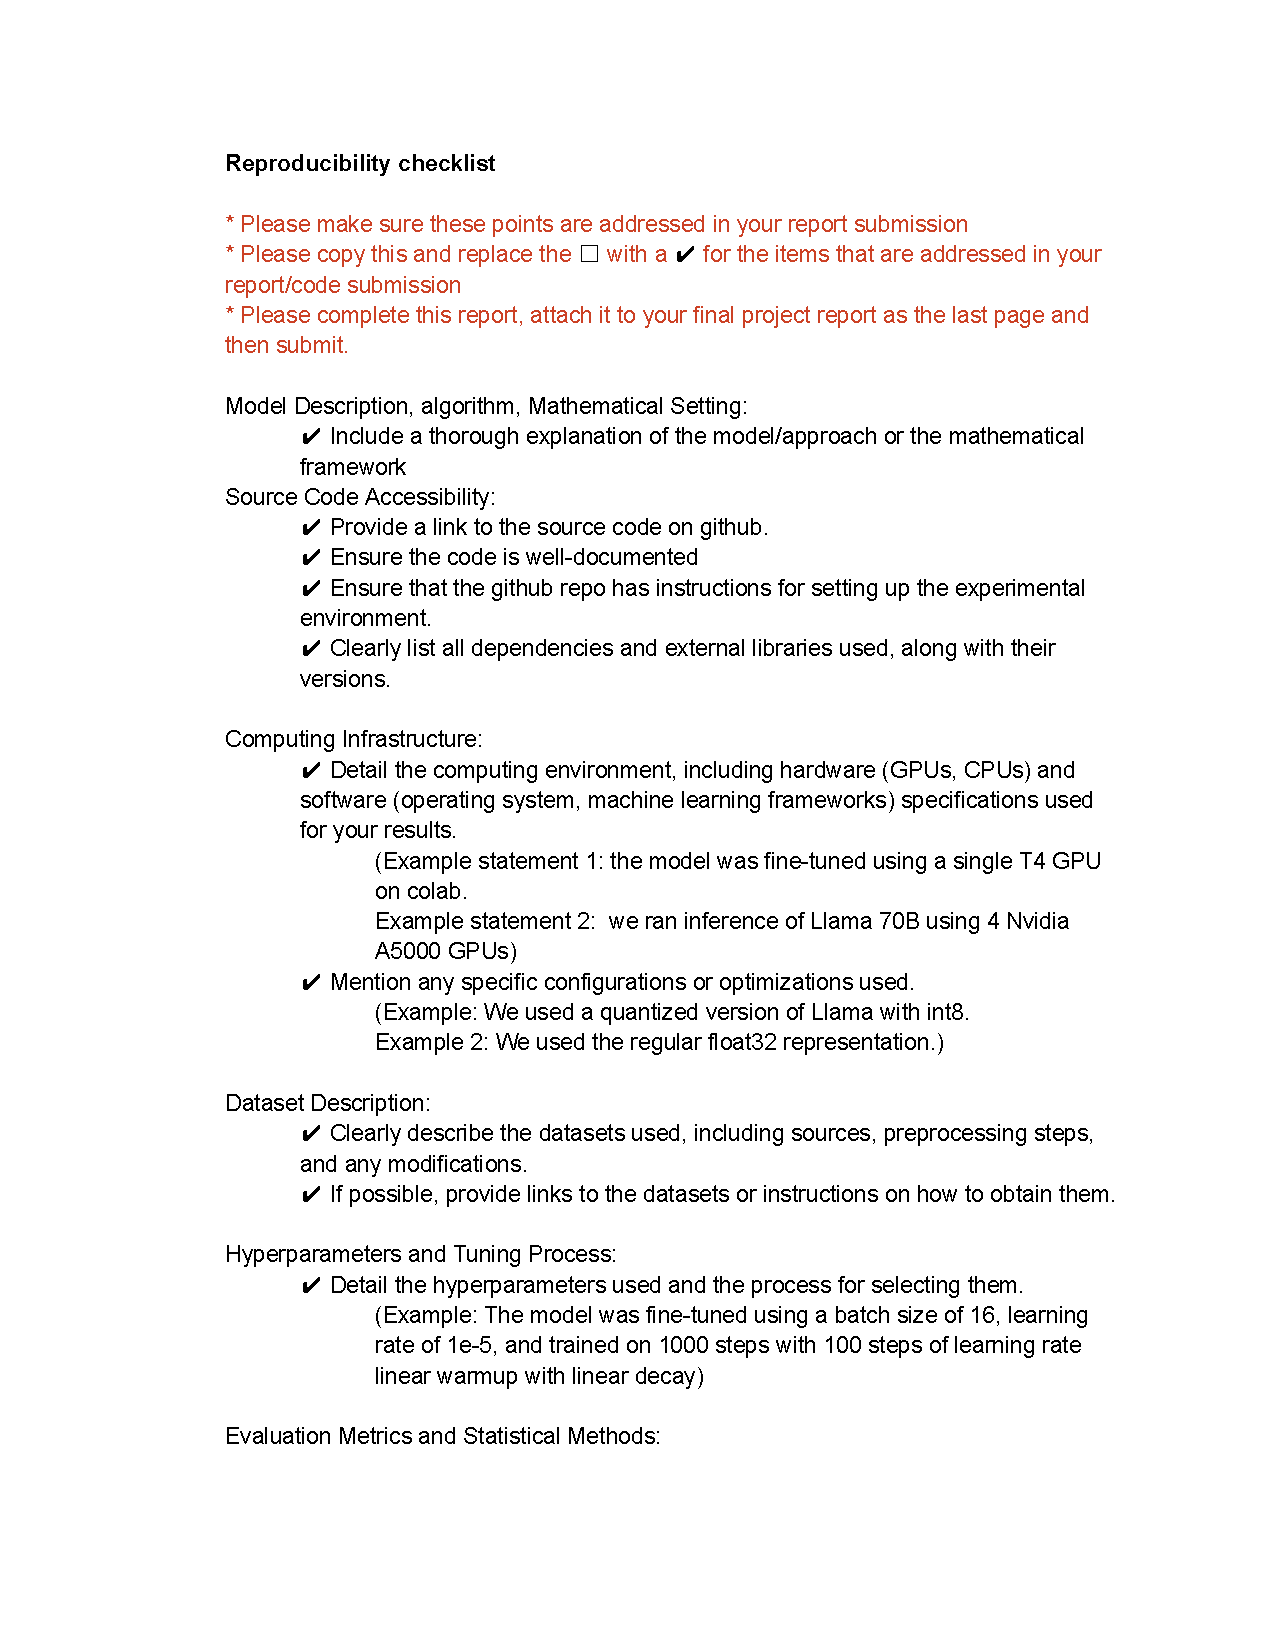
\includepdf[pages=-]{Reproducibility checklist.pdf}


%%%%%%%%%%%%%%%%%%%%%%%%%%%%%%%%%%%%%%%%%%%%%%%%%%%%%%%%%%%%


\end{document}